\documentclass[1p]{elsarticle_modified}
%\bibliographystyle{elsarticle-num}

%\usepackage[colorlinks]{hyperref}
%\usepackage{abbrmath_seonhwa} %\Abb, \Ascr, \Acal ,\Abf, \Afrak
\usepackage{amsfonts}
\usepackage{amssymb}
\usepackage{amsmath}
\usepackage{amsthm}
\usepackage{scalefnt}
\usepackage{amsbsy}
\usepackage{kotex}
\usepackage{caption}
\usepackage{subfig}
\usepackage{color}
\usepackage{graphicx}
\usepackage{xcolor} %% white, black, red, green, blue, cyan, magenta, yellow
\usepackage{float}
\usepackage{setspace}
\usepackage{hyperref}

\usepackage{tikz}
\usetikzlibrary{arrows}

\usepackage{multirow}
\usepackage{array} % fixed length table
\usepackage{hhline}

%%%%%%%%%%%%%%%%%%%%%
\makeatletter
\renewcommand*\env@matrix[1][\arraystretch]{%
	\edef\arraystretch{#1}%
	\hskip -\arraycolsep
	\let\@ifnextchar\new@ifnextchar
	\array{*\c@MaxMatrixCols c}}
\makeatother %https://tex.stackexchange.com/questions/14071/how-can-i-increase-the-line-spacing-in-a-matrix
%%%%%%%%%%%%%%%

\usepackage[normalem]{ulem}

\newcommand{\msout}[1]{\ifmmode\text{\sout{\ensuremath{#1}}}\else\sout{#1}\fi}
%SOURCE: \msout is \stkout macro in https://tex.stackexchange.com/questions/20609/strikeout-in-math-mode

\newcommand{\cancel}[1]{
	\ifmmode
	{\color{red}\msout{#1}}
	\else
	{\color{red}\sout{#1}}
	\fi
}

\newcommand{\add}[1]{
	{\color{blue}\uwave{#1}}
}

\newcommand{\replace}[2]{
	\ifmmode
	{\color{red}\msout{#1}}{\color{blue}\uwave{#2}}
	\else
	{\color{red}\sout{#1}}{\color{blue}\uwave{#2}}
	\fi
}

\newcommand{\Sol}{\mathcal{S}} %segment
\newcommand{\D}{D} %diagram
\newcommand{\A}{\mathcal{A}} %arc


%%%%%%%%%%%%%%%%%%%%%%%%%%%%%5 test

\def\sl{\operatorname{\textup{SL}}(2,\Cbb)}
\def\psl{\operatorname{\textup{PSL}}(2,\Cbb)}
\def\quan{\mkern 1mu \triangleright \mkern 1mu}

\theoremstyle{definition}
\newtheorem{thm}{Theorem}[section]
\newtheorem{prop}[thm]{Proposition}
\newtheorem{lem}[thm]{Lemma}
\newtheorem{ques}[thm]{Question}
\newtheorem{cor}[thm]{Corollary}
\newtheorem{defn}[thm]{Definition}
\newtheorem{exam}[thm]{Example}
\newtheorem{rmk}[thm]{Remark}
\newtheorem{alg}[thm]{Algorithm}

\newcommand{\I}{\sqrt{-1}}
\begin{document}

%\begin{frontmatter}
%
%\title{Boundary parabolic representations of knots up to 8 crossings}
%
%%% Group authors per affiliation:
%\author{Yunhi Cho} 
%\address{Department of Mathematics, University of Seoul, Seoul, Korea}
%\ead{yhcho@uos.ac.kr}
%
%
%\author{Seonhwa Kim} %\fnref{s_kim}}
%\address{Center for Geometry and Physics, Institute for Basic Science, Pohang, 37673, Korea}
%\ead{ryeona17@ibs.re.kr}
%
%\author{Hyuk Kim}
%\address{Department of Mathematical Sciences, Seoul National University, Seoul 08826, Korea}
%\ead{hyukkim@snu.ac.kr}
%
%\author{Seokbeom Yoon}
%\address{Department of Mathematical Sciences, Seoul National University, Seoul, 08826,  Korea}
%\ead{sbyoon15@snu.ac.kr}
%
%\begin{abstract}
%We find all boundary parabolic representation of knots up to 8 crossings.
%
%\end{abstract}
%\begin{keyword}
%    \MSC[2010] 57M25 
%\end{keyword}
%
%\end{frontmatter}

%\linenumbers
%\tableofcontents
%
\newcommand\colored[1]{\textcolor{white}{\rule[-0.35ex]{0.8em}{1.4ex}}\kern-0.8em\color{red} #1}%
%\newcommand\colored[1]{\textcolor{white}{ #1}\kern-2.17ex	\textcolor{white}{ #1}\kern-1.81ex	\textcolor{white}{ #1}\kern-2.15ex\color{red}#1	}

{\Large $\underline{11a_{177}~(K11a_{177})}$}

\setlength{\tabcolsep}{10pt}
\renewcommand{\arraystretch}{1.6}
\vspace{1cm}\begin{tabular}{m{100pt}>{\centering\arraybackslash}m{274pt}}
\multirow{5}{120pt}{
	\centering
	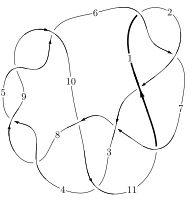
\includegraphics[width=112pt]{../../../GIT/diagram.site/Diagrams/png/426_11a_177.png}\\
\ \ \ A knot diagram\footnotemark}&
\allowdisplaybreaks
\textbf{Linearized knot diagam} \\
\cline{2-2}
 &
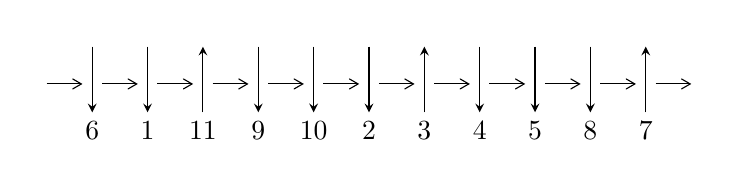
\begin{tikzpicture}[x=20pt, y=17pt]
	% nodes
	\node (C0) at (0, 0) {};
	\node (C1) at (1, 0) {};
	\node (C1U) at (1, +1) {};
	\node (C1D) at (1, -1) {6};

	\node (C2) at (2, 0) {};
	\node (C2U) at (2, +1) {};
	\node (C2D) at (2, -1) {1};

	\node (C3) at (3, 0) {};
	\node (C3U) at (3, +1) {};
	\node (C3D) at (3, -1) {11};

	\node (C4) at (4, 0) {};
	\node (C4U) at (4, +1) {};
	\node (C4D) at (4, -1) {9};

	\node (C5) at (5, 0) {};
	\node (C5U) at (5, +1) {};
	\node (C5D) at (5, -1) {10};

	\node (C6) at (6, 0) {};
	\node (C6U) at (6, +1) {};
	\node (C6D) at (6, -1) {2};

	\node (C7) at (7, 0) {};
	\node (C7U) at (7, +1) {};
	\node (C7D) at (7, -1) {3};

	\node (C8) at (8, 0) {};
	\node (C8U) at (8, +1) {};
	\node (C8D) at (8, -1) {4};

	\node (C9) at (9, 0) {};
	\node (C9U) at (9, +1) {};
	\node (C9D) at (9, -1) {5};

	\node (C10) at (10, 0) {};
	\node (C10U) at (10, +1) {};
	\node (C10D) at (10, -1) {8};

	\node (C11) at (11, 0) {};
	\node (C11U) at (11, +1) {};
	\node (C11D) at (11, -1) {7};
	\node (C12) at (12, 0) {};

	% arrows
	\draw[->,>={angle 60}]
	(C0) edge (C1) (C1) edge (C2) (C2) edge (C3) (C3) edge (C4) (C4) edge (C5) (C5) edge (C6) (C6) edge (C7) (C7) edge (C8) (C8) edge (C9) (C9) edge (C10) (C10) edge (C11) (C11) edge (C12) ;	\draw[->,>=stealth]
	(C1U) edge (C1D) (C2U) edge (C2D) (C3D) edge (C3U) (C4U) edge (C4D) (C5U) edge (C5D) (C6U) edge (C6D) (C7D) edge (C7U) (C8U) edge (C8D) (C9U) edge (C9D) (C10U) edge (C10D) (C11D) edge (C11U) ;
	\end{tikzpicture} \\
\hhline{~~} \\& 
\textbf{Solving Sequence} \\ \cline{2-2} 
 &
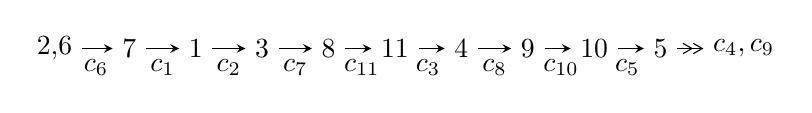
\begin{tikzpicture}[x=24pt, y=7pt]
	% node
	\node (A0) at (-1/8, 0) {2,6};
	\node (A1) at (1, 0) {7};
	\node (A2) at (2, 0) {1};
	\node (A3) at (3, 0) {3};
	\node (A4) at (4, 0) {8};
	\node (A5) at (5, 0) {11};
	\node (A6) at (6, 0) {4};
	\node (A7) at (7, 0) {9};
	\node (A8) at (8, 0) {10};
	\node (A9) at (9, 0) {5};
	\node (C1) at (1/2, -1) {$c_{6}$};
	\node (C2) at (3/2, -1) {$c_{1}$};
	\node (C3) at (5/2, -1) {$c_{2}$};
	\node (C4) at (7/2, -1) {$c_{7}$};
	\node (C5) at (9/2, -1) {$c_{11}$};
	\node (C6) at (11/2, -1) {$c_{3}$};
	\node (C7) at (13/2, -1) {$c_{8}$};
	\node (C8) at (15/2, -1) {$c_{10}$};
	\node (C9) at (17/2, -1) {$c_{5}$};
	\node (A10) at (41/4, 0) {$c_{4},c_{9}$};

	% edge
	\draw[->,>=stealth]	
	(A0) edge (A1) (A1) edge (A2) (A2) edge (A3) (A3) edge (A4) (A4) edge (A5) (A5) edge (A6) (A6) edge (A7) (A7) edge (A8) (A8) edge (A9) ;
	\draw[->>,>={angle 60}]	
	(A9) edge (A10);
\end{tikzpicture} \\ 

\end{tabular} \\

\footnotetext{
The image of knot diagram is generated by the software ``\textbf{Draw programme}" developed by Andrew Bartholomew(\url{http://www.layer8.co.uk/maths/draw/index.htm\#Running-draw}), where we modified some parts for our purpose(\url{https://github.com/CATsTAILs/LinksPainter}).
}\phantom \\ \newline 
\centering \textbf{Ideals for irreducible components\footnotemark of $X_{\text{par}}$} 
 
\begin{align*}
I^u_{1}&=\langle 
u^{48}- u^{47}+\cdots+2 u^2-1\rangle \\
\\
\end{align*}
\raggedright * 1 irreducible components of $\dim_{\mathbb{C}}=0$, with total 48 representations.\\
\footnotetext{All coefficients of polynomials are rational numbers. But the coefficients are sometimes approximated in decimal forms when there is not enough margin.}
\newpage
\renewcommand{\arraystretch}{1}
\centering \section*{I. $I^u_{1}= \langle u^{48}- u^{47}+\cdots+2 u^2-1 \rangle$}
\flushleft \textbf{(i) Arc colorings}\\
\begin{tabular}{m{7pt} m{180pt} m{7pt} m{180pt} }
\flushright $a_{2}=$&$\begin{pmatrix}0\\u\end{pmatrix}$ \\
\flushright $a_{6}=$&$\begin{pmatrix}1\\0\end{pmatrix}$ \\
\flushright $a_{7}=$&$\begin{pmatrix}1\\u^2\end{pmatrix}$ \\
\flushright $a_{1}=$&$\begin{pmatrix}u\\u\end{pmatrix}$ \\
\flushright $a_{3}=$&$\begin{pmatrix}- u^3\\- u^3+u\end{pmatrix}$ \\
\flushright $a_{8}=$&$\begin{pmatrix}u^8- u^6+u^4+1\\u^8-2 u^6+2 u^4\end{pmatrix}$ \\
\flushright $a_{11}=$&$\begin{pmatrix}u^3\\u^5- u^3+u\end{pmatrix}$ \\
\flushright $a_{4}=$&$\begin{pmatrix}u^{11}-2 u^9+2 u^7- u^3\\u^{13}-3 u^{11}+5 u^9-4 u^7+2 u^5- u^3+u\end{pmatrix}$ \\
\flushright $a_{9}=$&$\begin{pmatrix}u^{32}-7 u^{30}+\cdots+2 u^{12}+1\\u^{34}-8 u^{32}+\cdots+4 u^6+u^2\end{pmatrix}$ \\
\flushright $a_{10}=$&$\begin{pmatrix}u^{21}-4 u^{19}+9 u^{17}-12 u^{15}+12 u^{13}-10 u^{11}+9 u^9-6 u^7+3 u^5+u\\u^{21}-5 u^{19}+13 u^{17}-20 u^{15}+20 u^{13}-13 u^{11}+7 u^9-4 u^7+3 u^5- u^3+u\end{pmatrix}$ \\
\flushright $a_{5}=$&$\begin{pmatrix}- u^{42}+9 u^{40}+\cdots- u^2+1\\- u^{42}+10 u^{40}+\cdots+2 u^4- u^2\end{pmatrix}$\\ \flushright $a_{5}=$&$\begin{pmatrix}- u^{42}+9 u^{40}+\cdots- u^2+1\\- u^{42}+10 u^{40}+\cdots+2 u^4- u^2\end{pmatrix}$\\&\end{tabular}
\flushleft \textbf{(ii) Obstruction class $= -1$}\\~\\
\flushleft \textbf{(iii) Cusp Shapes $= -4 u^{46}+44 u^{44}+\cdots+8 u-6$}\\~\\
\newpage\renewcommand{\arraystretch}{1}
\flushleft \textbf{(iv) u-Polynomials at the component}\newline \\
\begin{tabular}{m{50pt}|m{274pt}}
Crossings & \hspace{64pt}u-Polynomials at each crossing \\
\hline $$\begin{aligned}c_{1},c_{6}\end{aligned}$$&$\begin{aligned}
&u^{48}- u^{47}+\cdots+2 u^2-1
\end{aligned}$\\
\hline $$\begin{aligned}c_{2}\end{aligned}$$&$\begin{aligned}
&u^{48}+23 u^{47}+\cdots+4 u+1
\end{aligned}$\\
\hline $$\begin{aligned}c_{3}\end{aligned}$$&$\begin{aligned}
&u^{48}+5 u^{47}+\cdots+440 u+41
\end{aligned}$\\
\hline $$\begin{aligned}c_{4},c_{5},c_{8}\\c_{9}\end{aligned}$$&$\begin{aligned}
&u^{48}- u^{47}+\cdots-2 u-1
\end{aligned}$\\
\hline $$\begin{aligned}c_{7}\end{aligned}$$&$\begin{aligned}
&u^{48}+u^{47}+\cdots-46 u-13
\end{aligned}$\\
\hline $$\begin{aligned}c_{10}\end{aligned}$$&$\begin{aligned}
&u^{48}-13 u^{47}+\cdots+248 u-23
\end{aligned}$\\
\hline $$\begin{aligned}c_{11}\end{aligned}$$&$\begin{aligned}
&u^{48}-3 u^{47}+\cdots+92 u-9
\end{aligned}$\\
\hline
\end{tabular}\\~\\
\newpage\renewcommand{\arraystretch}{1}
\flushleft \textbf{(v) Riley Polynomials at the component}\newline \\
\begin{tabular}{m{50pt}|m{274pt}}
Crossings & \hspace{64pt}Riley Polynomials at each crossing \\
\hline $$\begin{aligned}c_{1},c_{6}\end{aligned}$$&$\begin{aligned}
&y^{48}-23 y^{47}+\cdots-4 y+1
\end{aligned}$\\
\hline $$\begin{aligned}c_{2}\end{aligned}$$&$\begin{aligned}
&y^{48}+5 y^{47}+\cdots-12 y^2+1
\end{aligned}$\\
\hline $$\begin{aligned}c_{3}\end{aligned}$$&$\begin{aligned}
&y^{48}+17 y^{47}+\cdots-50264 y+1681
\end{aligned}$\\
\hline $$\begin{aligned}c_{4},c_{5},c_{8}\\c_{9}\end{aligned}$$&$\begin{aligned}
&y^{48}-55 y^{47}+\cdots-4 y+1
\end{aligned}$\\
\hline $$\begin{aligned}c_{7}\end{aligned}$$&$\begin{aligned}
&y^{48}-7 y^{47}+\cdots-6692 y+169
\end{aligned}$\\
\hline $$\begin{aligned}c_{10}\end{aligned}$$&$\begin{aligned}
&y^{48}-7 y^{47}+\cdots-5752 y+529
\end{aligned}$\\
\hline $$\begin{aligned}c_{11}\end{aligned}$$&$\begin{aligned}
&y^{48}+13 y^{47}+\cdots-8824 y+81
\end{aligned}$\\
\hline
\end{tabular}\\~\\
\newpage\flushleft \textbf{(vi) Complex Volumes and Cusp Shapes}
$$\begin{array}{c|c|c}  
\text{Solutions to }I^u_{1}& \I (\text{vol} + \sqrt{-1}CS) & \text{Cusp shape}\\
 \hline 
\begin{aligned}
u &= \phantom{-}0.950359\phantom{ +0.000000I}\end{aligned}
 & -7.68002\phantom{ +0.000000I} & -11.9160\phantom{ +0.000000I} \\ \hline\begin{aligned}
u &= \phantom{-}0.906245 + 0.560228 I\end{aligned}
 & -6.74396 + 1.23314 I & -7.83364 + 0.66658 I \\ \hline\begin{aligned}
u &= \phantom{-}0.906245 - 0.560228 I\end{aligned}
 & -6.74396 - 1.23314 I & -7.83364 - 0.66658 I \\ \hline\begin{aligned}
u &= \phantom{-}0.654967 + 0.639668 I\end{aligned}
 & -6.00272 - 5.94733 I & -6.48259 + 5.46714 I \\ \hline\begin{aligned}
u &= \phantom{-}0.654967 - 0.639668 I\end{aligned}
 & -6.00272 + 5.94733 I & -6.48259 - 5.46714 I \\ \hline\begin{aligned}
u &= -0.958032 + 0.533471 I\end{aligned}
 & \phantom{-}0.422311 + 0.763813 I & -4.66179 + 1.11475 I \\ \hline\begin{aligned}
u &= -0.958032 - 0.533471 I\end{aligned}
 & \phantom{-}0.422311 - 0.763813 I & -4.66179 - 1.11475 I \\ \hline\begin{aligned}
u &= -1.079460 + 0.276851 I\end{aligned}
 & -2.59116 + 0.36031 I & -7.93807 - 0.87976 I \\ \hline\begin{aligned}
u &= -1.079460 - 0.276851 I\end{aligned}
 & -2.59116 - 0.36031 I & -7.93807 + 0.87976 I \\ \hline\begin{aligned}
u &= -0.612298 + 0.617824 I\end{aligned}
 & \phantom{-}1.43265 + 3.79656 I & -3.21409 - 7.28282 I \\ \hline\begin{aligned}
u &= -0.612298 - 0.617824 I\end{aligned}
 & \phantom{-}1.43265 - 3.79656 I & -3.21409 + 7.28282 I \\ \hline\begin{aligned}
u &= \phantom{-}1.009290 + 0.540403 I\end{aligned}
 & \phantom{-}1.00278 - 4.13351 I & -2.80982 + 6.67284 I \\ \hline\begin{aligned}
u &= \phantom{-}1.009290 - 0.540403 I\end{aligned}
 & \phantom{-}1.00278 + 4.13351 I & -2.80982 - 6.67284 I \\ \hline\begin{aligned}
u &= \phantom{-}1.118000 + 0.248646 I\end{aligned}
 & -4.32121 + 2.98517 I & -12.02372 - 4.32221 I \\ \hline\begin{aligned}
u &= \phantom{-}1.118000 - 0.248646 I\end{aligned}
 & -4.32121 - 2.98517 I & -12.02372 + 4.32221 I \\ \hline\begin{aligned}
u &= \phantom{-}1.109880 + 0.332950 I\end{aligned}
 & -5.19194 - 3.05995 I & -13.8975 + 5.0529 I \\ \hline\begin{aligned}
u &= \phantom{-}1.109880 - 0.332950 I\end{aligned}
 & -5.19194 + 3.05995 I & -13.8975 - 5.0529 I \\ \hline\begin{aligned}
u &= \phantom{-}0.320233 + 0.770338 I\end{aligned}
 & -7.65892 + 8.01718 I & -7.88582 - 4.62371 I \\ \hline\begin{aligned}
u &= \phantom{-}0.320233 - 0.770338 I\end{aligned}
 & -7.65892 - 8.01718 I & -7.88582 + 4.62371 I \\ \hline\begin{aligned}
u &= -1.144450 + 0.242249 I\end{aligned}
 & -12.21720 - 5.14750 I & -14.0897 + 2.5540 I \\ \hline\begin{aligned}
u &= -1.144450 - 0.242249 I\end{aligned}
 & -12.21720 + 5.14750 I & -14.0897 - 2.5540 I \\ \hline\begin{aligned}
u &= -0.466321 + 0.682642 I\end{aligned}
 & -3.08169 - 1.06539 I & -4.15324 + 0.48438 I \\ \hline\begin{aligned}
u &= -0.466321 - 0.682642 I\end{aligned}
 & -3.08169 + 1.06539 I & -4.15324 - 0.48438 I \\ \hline\begin{aligned}
u &= \phantom{-}0.541320 + 0.609466 I\end{aligned}
 & \phantom{-}2.38297 - 0.42475 I & \phantom{-}0.428840 - 0.154422 I \\ \hline\begin{aligned}
u &= \phantom{-}0.541320 - 0.609466 I\end{aligned}
 & \phantom{-}2.38297 + 0.42475 I & \phantom{-}0.428840 + 0.154422 I \\ \hline\begin{aligned}
u &= -0.330482 + 0.744977 I\end{aligned}
 & \phantom{-}0.08939 - 5.70419 I & -5.22111 + 6.43741 I \\ \hline\begin{aligned}
u &= -0.330482 - 0.744977 I\end{aligned}
 & \phantom{-}0.08939 + 5.70419 I & -5.22111 - 6.43741 I \\ \hline\begin{aligned}
u &= -1.143670 + 0.342258 I\end{aligned}
 & -13.35450 + 4.59259 I & -15.0956 - 3.6225 I \\ \hline\begin{aligned}
u &= -1.143670 - 0.342258 I\end{aligned}
 & -13.35450 - 4.59259 I & -15.0956 + 3.6225 I \\ \hline\begin{aligned}
u &= -1.050160 + 0.567901 I\end{aligned}
 & -4.79213 + 5.90007 I & -7.32134 - 5.68166 I\\
 \hline 
 \end{array}$$\newpage$$\begin{array}{c|c|c}  
\text{Solutions to }I^u_{1}& \I (\text{vol} + \sqrt{-1}CS) & \text{Cusp shape}\\
 \hline 
\begin{aligned}
u &= -1.050160 - 0.567901 I\end{aligned}
 & -4.79213 - 5.90007 I & -7.32134 + 5.68166 I \\ \hline\begin{aligned}
u &= \phantom{-}0.346872 + 0.703599 I\end{aligned}
 & \phantom{-}1.51359 + 2.15734 I & -1.22557 - 1.03658 I \\ \hline\begin{aligned}
u &= \phantom{-}0.346872 - 0.703599 I\end{aligned}
 & \phantom{-}1.51359 - 2.15734 I & -1.22557 + 1.03658 I \\ \hline\begin{aligned}
u &= -1.108460 + 0.518737 I\end{aligned}
 & -3.93668 + 4.44888 I & -11.97527 - 2.81455 I \\ \hline\begin{aligned}
u &= -1.108460 - 0.518737 I\end{aligned}
 & -3.93668 - 4.44888 I & -11.97527 + 2.81455 I \\ \hline\begin{aligned}
u &= \phantom{-}1.107780 + 0.553922 I\end{aligned}
 & -0.69945 - 6.98562 I & -4.89380 + 5.04107 I \\ \hline\begin{aligned}
u &= \phantom{-}1.107780 - 0.553922 I\end{aligned}
 & -0.69945 + 6.98562 I & -4.89380 - 5.04107 I \\ \hline\begin{aligned}
u &= \phantom{-}1.134660 + 0.506389 I\end{aligned}
 & -12.24490 - 3.33222 I & -13.52387 + 3.39581 I \\ \hline\begin{aligned}
u &= \phantom{-}1.134660 - 0.506389 I\end{aligned}
 & -12.24490 + 3.33222 I & -13.52387 - 3.39581 I \\ \hline\begin{aligned}
u &= -1.122190 + 0.562178 I\end{aligned}
 & -2.22657 + 10.65640 I & -8.51135 - 10.01533 I \\ \hline\begin{aligned}
u &= -1.122190 - 0.562178 I\end{aligned}
 & -2.22657 - 10.65640 I & -8.51135 + 10.01533 I \\ \hline\begin{aligned}
u &= \phantom{-}1.132630 + 0.566501 I\end{aligned}
 & -10.0472 - 13.0450 I & -11.01452 + 8.25936 I \\ \hline\begin{aligned}
u &= \phantom{-}1.132630 - 0.566501 I\end{aligned}
 & -10.0472 + 13.0450 I & -11.01452 - 8.25936 I \\ \hline\begin{aligned}
u &= \phantom{-}0.180677 + 0.698013 I\end{aligned}
 & -9.54554 - 1.19929 I & -10.13609 + 0.35134 I \\ \hline\begin{aligned}
u &= \phantom{-}0.180677 - 0.698013 I\end{aligned}
 & -9.54554 + 1.19929 I & -10.13609 - 0.35134 I \\ \hline\begin{aligned}
u &= -0.240215 + 0.625865 I\end{aligned}
 & -1.54227 + 0.02620 I & -8.94545 - 1.26503 I \\ \hline\begin{aligned}
u &= -0.240215 - 0.625865 I\end{aligned}
 & -1.54227 - 0.02620 I & -8.94545 + 1.26503 I \\ \hline\begin{aligned}
u &= -0.563965\phantom{ +0.000000I}\end{aligned}
 & -0.872825\phantom{ +0.000000I} & -11.2330\phantom{ +0.000000I}\\
 \hline 
 \end{array}$$\newpage
\newpage\renewcommand{\arraystretch}{1}
\centering \section*{ II. u-Polynomials}
\begin{tabular}{m{50pt}|m{274pt}}
Crossings & \hspace{64pt}u-Polynomials at each crossing \\
\hline $$\begin{aligned}c_{1},c_{6}\end{aligned}$$&$\begin{aligned}
&u^{48}- u^{47}+\cdots+2 u^2-1
\end{aligned}$\\
\hline $$\begin{aligned}c_{2}\end{aligned}$$&$\begin{aligned}
&u^{48}+23 u^{47}+\cdots+4 u+1
\end{aligned}$\\
\hline $$\begin{aligned}c_{3}\end{aligned}$$&$\begin{aligned}
&u^{48}+5 u^{47}+\cdots+440 u+41
\end{aligned}$\\
\hline $$\begin{aligned}c_{4},c_{5},c_{8}\\c_{9}\end{aligned}$$&$\begin{aligned}
&u^{48}- u^{47}+\cdots-2 u-1
\end{aligned}$\\
\hline $$\begin{aligned}c_{7}\end{aligned}$$&$\begin{aligned}
&u^{48}+u^{47}+\cdots-46 u-13
\end{aligned}$\\
\hline $$\begin{aligned}c_{10}\end{aligned}$$&$\begin{aligned}
&u^{48}-13 u^{47}+\cdots+248 u-23
\end{aligned}$\\
\hline $$\begin{aligned}c_{11}\end{aligned}$$&$\begin{aligned}
&u^{48}-3 u^{47}+\cdots+92 u-9
\end{aligned}$\\
\hline
\end{tabular}\newpage\renewcommand{\arraystretch}{1}
\centering \section*{ III. Riley Polynomials}
\begin{tabular}{m{50pt}|m{274pt}}
Crossings & \hspace{64pt}Riley Polynomials at each crossing \\
\hline $$\begin{aligned}c_{1},c_{6}\end{aligned}$$&$\begin{aligned}
&y^{48}-23 y^{47}+\cdots-4 y+1
\end{aligned}$\\
\hline $$\begin{aligned}c_{2}\end{aligned}$$&$\begin{aligned}
&y^{48}+5 y^{47}+\cdots-12 y^2+1
\end{aligned}$\\
\hline $$\begin{aligned}c_{3}\end{aligned}$$&$\begin{aligned}
&y^{48}+17 y^{47}+\cdots-50264 y+1681
\end{aligned}$\\
\hline $$\begin{aligned}c_{4},c_{5},c_{8}\\c_{9}\end{aligned}$$&$\begin{aligned}
&y^{48}-55 y^{47}+\cdots-4 y+1
\end{aligned}$\\
\hline $$\begin{aligned}c_{7}\end{aligned}$$&$\begin{aligned}
&y^{48}-7 y^{47}+\cdots-6692 y+169
\end{aligned}$\\
\hline $$\begin{aligned}c_{10}\end{aligned}$$&$\begin{aligned}
&y^{48}-7 y^{47}+\cdots-5752 y+529
\end{aligned}$\\
\hline $$\begin{aligned}c_{11}\end{aligned}$$&$\begin{aligned}
&y^{48}+13 y^{47}+\cdots-8824 y+81
\end{aligned}$\\
\hline
\end{tabular}
\vskip 2pc
\end{document}